\documentclass[aspectratio=169,10pt]{beamer}

% Modern theme
\usetheme{Madrid}
\usecolortheme{seahorse}
\useinnertheme{rectangles}
\useoutertheme{infolines}

% Packages for modern look
\usepackage[utf8]{inputenc}
\usepackage[T1]{fontenc}
\usepackage[english,hungarian]{babel}
\usepackage{amsmath,amssymb}
\usepackage{graphicx}
\usepackage{tikz}
\usepackage{pgfplots}
\usepackage{listings}
\usepackage{xcolor}
\usepackage{hyperref}
\usepackage{fontawesome5}

% Code highlighting
\lstset{
    language=Python,
    basicstyle=\ttfamily\footnotesize,
    keywordstyle=\color{blue},
    commentstyle=\color{green!60!black},
    stringstyle=\color{red},
    numbers=left,
    numberstyle=\tiny,
    frame=single,
    breaklines=true,
    showstringspaces=false
}

% Custom colors
\definecolor{virtplc-blue}{RGB}{0,123,255}
\definecolor{virtplc-green}{RGB}{40,167,69}
\definecolor{virtplc-orange}{RGB}{255,193,7}
\definecolor{virtplc-red}{RGB}{220,53,69}

% Title page info
\title[VirtPLC]{VirtPLC - AI Hajtotta Ipari Automatizálási Platform}
\subtitle{Digitális Ikrek Intelligens Raktárak Számára}
\author[VirtPLC Csapat]{VirtPLC Fejlesztő Csapat}
\institute[Accenture Challenge]{Accenture Magyarország}
\date{\today}

% Custom commands
\newcommand{\highlight}[1]{\textcolor{virtplc-blue}{\textbf{#1}}}
\newcommand{\tech}[1]{\texttt{#1}}
\newcommand{\icon}[1]{\faIcon{#1}}

\begin{document}

% Title slide
\begin{frame}[plain]
    \titlepage
\end{frame}

% Agenda
\begin{frame}{Napirend}
    \tableofcontents
\end{frame}

\section{Bevezetés}

\begin{frame}{Mi a VirtPLC?}
    \begin{columns}[c]
        \column{0.6\textwidth}
        \begin{itemize}
            \item \highlight{Komplex ipari automatizálási platform}
            \item \highlight{Virtuális PLC ökoszisztéma} gyári automatizáláshoz
            \item \highlight{Mikroszolgáltatás-alapú megoldás} monitoringhoz, vezérléshez és optimalizáláshoz
            \item \highlight{AI-fokozott prediktív karbantartás} és valós idejű adatelemzés
        \end{itemize}
        
        \column{0.4\textwidth}
        \begin{figure}
            \centering
            \includegraphics[width=\textwidth]{placeholder_architecture_diagram.png}
            \caption{Rendszer architektúra áttekintés}
        \end{figure}
    \end{columns}
\end{frame}

\begin{frame}{A Kihívás}
    \begin{alertblock}{Ipari Valóság}
        \begin{itemize}
            \item \highlight{28 különböző szenzor} minden gépen
            \item \highlight{Valós idejű monitoring} kritikus fontosságú
            \item \highlight{Prediktív karbantartás} költségmegtakarítás
            \item \highlight{Operátor túlterhelés} információáradattal
        \end{itemize}
    \end{alertblock}
    
    \vspace{0.5cm}
    
    \begin{block}{VirtPLC Megoldás}
        \highlight{AI intelligens szűrés + valós idejű vizualizáció}
    \end{block}
\end{frame}

\section{Architektúra}

\begin{frame}{Mikroszolgáltatás Architektúra}
    \begin{figure}
        \centering
        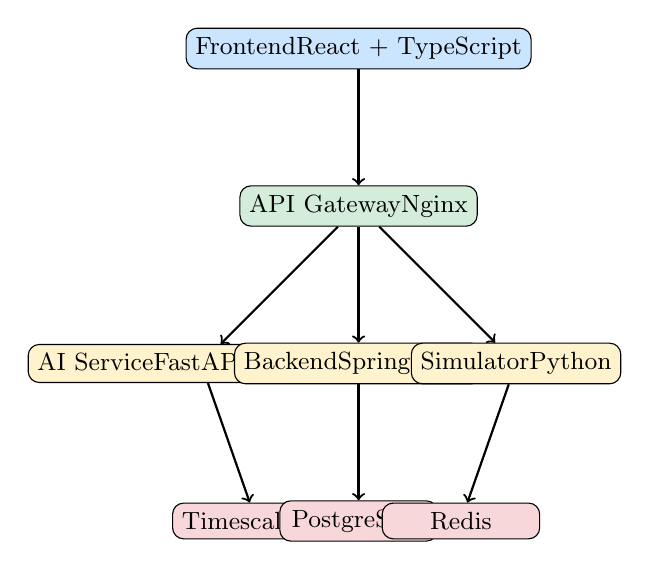
\begin{tikzpicture}[node distance=2cm, auto, font=\small]
            % Frontend layer
            \node[draw, fill=virtplc-blue!20, rounded corners, minimum width=3cm] (frontend) {Frontend\\React + TypeScript};
            
            % API Gateway layer
            \node[draw, fill=virtplc-green!20, rounded corners, minimum width=3cm, below of=frontend] (gateway) {API Gateway\\Nginx};
            
            % Services layer
            \node[draw, fill=virtplc-orange!20, rounded corners, minimum width=2.5cm, below of=gateway, xshift=-2cm] (ai) {AI Service\\FastAPI + Ollama};
            \node[draw, fill=virtplc-orange!20, rounded corners, minimum width=2.5cm, below of=gateway] (backend) {Backend\\Spring Boot};
            \node[draw, fill=virtplc-orange!20, rounded corners, minimum width=2.5cm, below of=gateway, xshift=2cm] (simulator) {Simulator\\Python};
            
            % Data layer
            \node[draw, fill=virtplc-red!20, rounded corners, minimum width=2cm, below of=ai, xshift=0.7cm] (timescale) {TimescaleDB};
            \node[draw, fill=virtplc-red!20, rounded corners, minimum width=2cm, below of=backend] (postgres) {PostgreSQL};
            \node[draw, fill=virtplc-red!20, rounded corners, minimum width=2cm, below of=simulator, xshift=-0.7cm] (redis) {Redis};
            
            % Connections
            \draw[->, thick] (frontend) -- (gateway);
            \draw[->, thick] (gateway) -- (ai);
            \draw[->, thick] (gateway) -- (backend);
            \draw[->, thick] (gateway) -- (simulator);
            \draw[->, thick] (ai) -- (timescale);
            \draw[->, thick] (backend) -- (postgres);
            \draw[->, thick] (simulator) -- (redis);
        \end{tikzpicture}
        \caption{VirtPLC mikroszolgáltatás architektúra}
    \end{figure}
\end{frame}

\begin{frame}{Technológiai Stack - Indoklás}
    \begin{columns}[c]
        \column{0.5\textwidth}
        \begin{block}{Frontend}
            \begin{itemize}
                \item \tech{React + TypeScript + Vite}
                \item \highlight{Modern DX} - gyors fejlesztés
                \item \highlight{Type Safety} - kevesebb bug
                \item \highlight{Component Library} - konzisztens UI
            \end{itemize}
        \end{block}
        
        \column{0.5\textwidth}
        \begin{block}{Backend}
            \begin{itemize}
                \item \tech{Java Spring Boot}
                \item \highlight{Enterprise Grade} - megbízhatóság
                \item \highlight{OPC-UA Support} - ipari szabvány
                \item \highlight{JWT Security} - biztonság
            \end{itemize}
        \end{block}
    \end{columns}
\end{frame}

\begin{frame}{AI Stack - Miért Ez A Kombináció?}
    \begin{columns}[c]
        \column{0.5\textwidth}
        \begin{block}{FastAPI + Python}
            \begin{itemize}
                \item \highlight{Async First} - nagy teljesítmény
                \item \highlight{Auto Documentation} - OpenAPI
                \item \highlight{Python Ecosystem} - AI/ML könyvtárak
                \item \highlight{Rapid Prototyping} - gyors iteráció
            \end{itemize}
        \end{block}
        
        \column{0.5\textwidth}
        \begin{block}{Ollama + LLaMA}
            \begin{itemize}
                \item \highlight{Offline First} - adatvédelem
                \item \highlight{Local Deployment} - költséghatékonyság
                \item \highlight{Open Source} - transzparencia
                \item \highlight{Custom Fine-tuning} - domain specifikus
            \end{itemize}
        \end{block}
    \end{columns}
\end{frame}

\begin{frame}{Adatbázis Stratégia}
    \begin{columns}[c]
        \column{0.33\textwidth}
        \begin{block}{PostgreSQL}
            \begin{itemize}
                \item Üzleti adatok
                \item Konfigurációk
                \item Felhasználók
                \item ACID compliance
            \end{itemize}
        \end{block}
        
        \column{0.33\textwidth}
        \begin{block}{TimescaleDB}
            \begin{itemize}
                \item Idősor adatok
                \item Szenzor értékek
                \item Nagy teljesítmény
                \item Automatikus particionálás
            \end{itemize}
        \end{block}
        
        \column{0.33\textwidth}
        \begin{block}{Redis}
            \begin{itemize}
                \item Cache layer
                \item Session management
                \item Message queue
                \item Valós idejű pub/sub
            \end{itemize}
        \end{block}
    \end{columns}
\end{frame}

\section{Kulcs Funkciók}

\begin{frame}{AI-Powered Intelligens Elemzés}
    \begin{columns}[c]
        \column{0.6\textwidth}
        \begin{itemize}
            \item \highlight{NLP Chat Interface} - természetes nyelv
            \item \highlight{Intent Analysis} - kontextus megértés
            \item \highlight{Automatikus Szűrés} - releváns adatok csak
            \item \highlight{Predictive Maintenance} - prediktív karbantartás
            \item \highlight{Anomaly Detection} - anomália detektálás
        \end{itemize}
        
        \column{0.4\textwidth}
        \begin{figure}
            \centering
            \includegraphics[width=\textwidth]{placeholder_ai_demo.png}
            \caption{AI chat demonstráció}
        \end{figure}
    \end{columns}
\end{frame}

\begin{frame}{Valós Idejű Monitoring Dashboard}
    \begin{figure}
        \centering
        \includegraphics[width=\textwidth]{placeholder_dashboard_screenshot.png}
        \caption{VirtPLC HMI Dashboard}
    \end{figure}
    
    \begin{itemize}
        \item \highlight{28 szenzor} helyett intelligens szűrés
        \item \highlight{WebSocket streaming} - <2s latency
        \item \highlight{Drag-and-drop} dashboard builder
        \item \highlight{Export funkcionalitás} - PDF/CSV
        \item \highlight{Role-based access} - biztonság
    \end{itemize}
\end{frame}

\begin{frame}{OPC-UA Ipari Kommunikáció}
    \begin{columns}[c]
        \column{0.5\textwidth}
        \begin{block}{OPC-UA Server}
            \begin{itemize}
                \item Ipari szabvány protokoll
                \item Biztonságos kommunikáció
                \item Namespace management
                \item Tag synchronization
            \end{itemize}
        \end{block}
        
        \column{0.5\textwidth}
        \begin{block}{PLC Simulator}
            \begin{itemize}
                \item Virtuális PLC környezet
                \item Fejlesztési tesztelés
                \item Production-ready
                \item MQTT integráció
            \end{itemize}
        \end{block}
    \end{columns}
\end{frame}

\section{Üzleti Érték}

\begin{frame}{ROI és Költségmegtakarítás}
    \begin{columns}[c]
        \column{0.5\textwidth}
        \begin{block}{Költségmegtakarítás}
            \begin{itemize}
                \item \highlight{30-50\%} karbantartási költség csökkentés
                \item \highlight{Predictive maintenance} - tervezett leállások
                \item \highlight{Anomaly detection} - korai beavatkozás
                \item \highlight{Operátor efficiency} - intelligens szűrés
            \end{itemize}
        \end{block}
        
        \column{0.5\textwidth}
        \begin{figure}
            \centering
            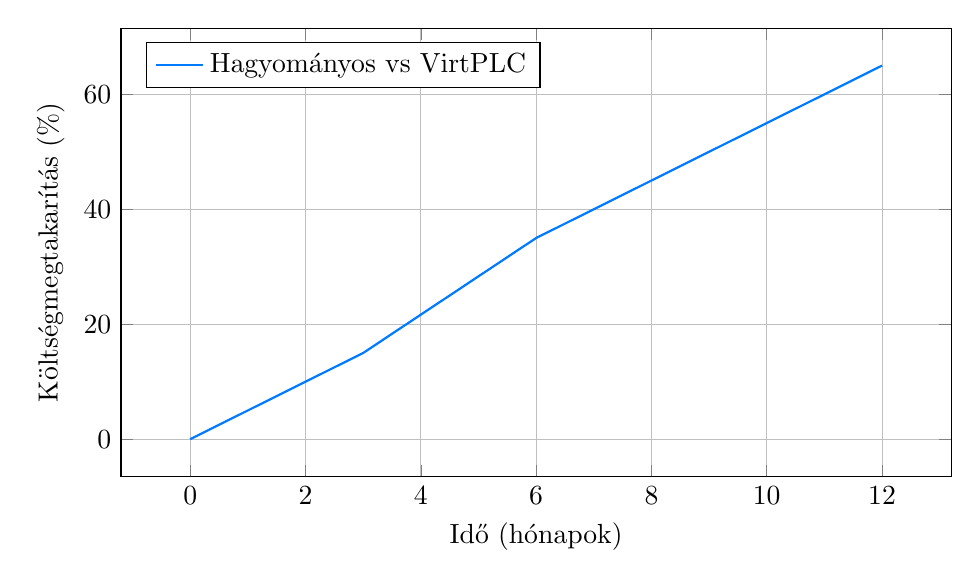
\begin{tikzpicture}
                \begin{axis}[
                    width=\textwidth,
                    height=0.6\textwidth,
                    xlabel={Idő (hónapok)},
                    ylabel={Költségmegtakarítás (\%)},
                    grid=major,
                    legend pos=north west
                ]
                \addplot[virtplc-blue, thick] coordinates {
                    (0,0) (3,15) (6,35) (9,50) (12,65)
                };
                \legend{Hagyományos vs VirtPLC}
                \end{axis}
            \end{tikzpicture}
            \caption{ROI görbe - 12 hónapos payback}
        \end{figure}
    \end{columns}
\end{frame}

\begin{frame}{Versenyelőnyök}
    \begin{alertblock}{Mi Különböztet Meg Minket?}
        \begin{itemize}
            \item \highlight{AI-First Approach} - nem csak monitoring
            \item \highlight{Open Source Core} - transzparencia és közösség
            \item \highlight{Cloud-Ready} - Kubernetes deployment
            \item \highlight{Industry 4.0 Compliant} - jövőbiztos
            \item \highlight{Hungarian Innovation} - helyi szakértelem
        \end{itemize}
    \end{alertblock}
\end{frame}

\section{Kooperációs Lehetőségek}

\begin{frame}{Partnership Modellek}
    \begin{columns}[c]
        \column{0.5\textwidth}
        \begin{block}{Technikai Partnerség}
            \begin{itemize}
                \item \highlight{Joint Development} - egyedi funkciók
                \item \highlight{Integration Services} - meglévő rendszerek
                \item \highlight{Training \& Support} - know-how transzfer
                \item \highlight{Custom AI Models} - domain specifikus
            \end{itemize}
        \end{block}
        
        \column{0.5\textwidth}
        \begin{block}{Üzleti Partnerség}
            \begin{itemize}
                \item \highlight{Pilóta Projektek} - proof of concept
                \item \highlight{White-label Solution} - saját branding
                \item \highlight{Market Expansion} - új piacok
                \item \highlight{Investment Opportunities} - növekedés együtt
            \end{itemize}
        \end{block}
    \end{columns}
\end{frame}

\begin{frame}{Célpiacok és Alkalmazási Területek}
    \begin{columns}[c]
        \column{0.5\textwidth}
        \begin{itemize}
            \item \icon{industry} \highlight{Gyártóipar} - összes vertikum
            \item \icon{truck} \highlight{Logisztika} - raktárak, disztribúció
            \item \icon{bolt} \highlight{Energetika} - erőművek, hálózatok
            \item \icon{ship} \highlight{Olaj és gáz} - finomítók, terminálok
            \item \icon{building} \highlight{Épületgazdálkodás} - smart buildings
        \end{itemize}
        
        \column{0.5\textwidth}
        \begin{figure}
            \centering
            \includegraphics[width=\textwidth]{placeholder_market_opportunities.png}
            \caption{Piaci lehetőségek}
        \end{figure}
    \end{columns}
\end{frame}

\section{Technikai Demó}

\begin{frame}{Élő Demonstráció}
    \begin{columns}[c]
        \column{0.6\textwidth}
        \begin{block}{Demo Forgatókönyv}
            \begin{enumerate}
                \item \highlight{AI Chat} - "Mutasd a motor hőmérséklet adatokat"
                \item \highlight{Intelligens Szűrés} - csak releváns szenzorok
                \item \highlight{Valós Idejű Chart} - automatikus vizualizáció
                \item \highlight{Predictive Alert} - karbantartási javaslat
            \end{enumerate}
        \end{block}
        
        \column{0.4\textwidth}
        \begin{figure}
            \centering
            \includegraphics[width=\textwidth]{placeholder_live_demo.png}
            \caption{Élő rendszer demonstráció}
        \end{figure}
    \end{columns}
\end{frame}

\begin{frame}{Roadmap 2026}
    \begin{columns}[c]
        \column{0.5\textwidth}
        \begin{block}{Q1 2026 - Enterprise Features}
            \begin{itemize}
                \item Multi-tenant architecture
                \item Advanced user management
                \item Custom dashboard templates
                \item Integration APIs
            \end{itemize}
        \end{block}
        
        \column{0.5\textwidth}
        \begin{block}{Q2 2026 - AI Enhancement}
            \begin{itemize}
                \item Fine-tuned industry models
                \item Predictive maintenance ML
                \item Computer vision integration
                \item Advanced analytics
            \end{itemize}
        \end{block}
    \end{columns}
\end{frame}

\begin{frame}{Hosszú Távú Vízió}
    \begin{block}{Industry 4.0 Platform}
        \begin{itemize}
            \item \highlight{Digital Twin Ecosystem} - teljes gyári digitalizáció
            \item \highlight{AI-Driven Optimization} - automatizált folyamatok
            \item \highlight{Edge Computing} - helyi intelligencia
            \item \highlight{5G Integration} - ultra-low latency
            \item \highlight{Sustainability Focus} - energia optimalizáció
        \end{itemize}
    \end{block}
\end{frame}

\begin{frame}{Hosszú Távú Vízió}
    \begin{block}{Industry 4.0 Platform}
        \begin{itemize}
            \item \highlight{Digital Twin Ecosystem} - teljes gyári digitalizáció
            \item \highlight{AI-Driven Optimization} - automatizált folyamatok
            \item \highlight{Edge Computing} - helyi intelligencia
            \item \highlight{5G Integration} - ultra-low latency
            \item \highlight{Sustainability Focus} - energia optimalizáció
        \end{itemize}
    \end{block}
\end{frame}

\section{Kapcsolat}

\begin{frame}{Köszönjük a Figyelmet!}
    \begin{center}
        \huge \highlight{Kérdések?}
        
        \vspace{1cm}
        
        \Large \highlight{VirtPLC - Az Ipari Jövő Ma}
        
        \vspace{1cm}
        
        \begin{figure}
            \centering
            \includegraphics[width=0.8\textwidth]{placeholder_virtplc_logo.png}
        \end{figure}
    \end{center}
\end{frame}

\end{document}